% Options for packages loaded elsewhere
\PassOptionsToPackage{unicode}{hyperref}
\PassOptionsToPackage{hyphens}{url}
\PassOptionsToPackage{dvipsnames,svgnames,x11names}{xcolor}
%
\documentclass[
  letterpaper,
  DIV=11,
  numbers=noendperiod]{scrartcl}

\usepackage{amsmath,amssymb}
\usepackage{iftex}
\ifPDFTeX
  \usepackage[T1]{fontenc}
  \usepackage[utf8]{inputenc}
  \usepackage{textcomp} % provide euro and other symbols
\else % if luatex or xetex
  \usepackage{unicode-math}
  \defaultfontfeatures{Scale=MatchLowercase}
  \defaultfontfeatures[\rmfamily]{Ligatures=TeX,Scale=1}
\fi
\usepackage{lmodern}
\ifPDFTeX\else  
    % xetex/luatex font selection
\fi
% Use upquote if available, for straight quotes in verbatim environments
\IfFileExists{upquote.sty}{\usepackage{upquote}}{}
\IfFileExists{microtype.sty}{% use microtype if available
  \usepackage[]{microtype}
  \UseMicrotypeSet[protrusion]{basicmath} % disable protrusion for tt fonts
}{}
\makeatletter
\@ifundefined{KOMAClassName}{% if non-KOMA class
  \IfFileExists{parskip.sty}{%
    \usepackage{parskip}
  }{% else
    \setlength{\parindent}{0pt}
    \setlength{\parskip}{6pt plus 2pt minus 1pt}}
}{% if KOMA class
  \KOMAoptions{parskip=half}}
\makeatother
\usepackage{xcolor}
\setlength{\emergencystretch}{3em} % prevent overfull lines
\setcounter{secnumdepth}{5}
% Make \paragraph and \subparagraph free-standing
\ifx\paragraph\undefined\else
  \let\oldparagraph\paragraph
  \renewcommand{\paragraph}[1]{\oldparagraph{#1}\mbox{}}
\fi
\ifx\subparagraph\undefined\else
  \let\oldsubparagraph\subparagraph
  \renewcommand{\subparagraph}[1]{\oldsubparagraph{#1}\mbox{}}
\fi


\providecommand{\tightlist}{%
  \setlength{\itemsep}{0pt}\setlength{\parskip}{0pt}}\usepackage{longtable,booktabs,array}
\usepackage{calc} % for calculating minipage widths
% Correct order of tables after \paragraph or \subparagraph
\usepackage{etoolbox}
\makeatletter
\patchcmd\longtable{\par}{\if@noskipsec\mbox{}\fi\par}{}{}
\makeatother
% Allow footnotes in longtable head/foot
\IfFileExists{footnotehyper.sty}{\usepackage{footnotehyper}}{\usepackage{footnote}}
\makesavenoteenv{longtable}
\usepackage{graphicx}
\makeatletter
\def\maxwidth{\ifdim\Gin@nat@width>\linewidth\linewidth\else\Gin@nat@width\fi}
\def\maxheight{\ifdim\Gin@nat@height>\textheight\textheight\else\Gin@nat@height\fi}
\makeatother
% Scale images if necessary, so that they will not overflow the page
% margins by default, and it is still possible to overwrite the defaults
% using explicit options in \includegraphics[width, height, ...]{}
\setkeys{Gin}{width=\maxwidth,height=\maxheight,keepaspectratio}
% Set default figure placement to htbp
\makeatletter
\def\fps@figure{htbp}
\makeatother

\KOMAoption{captions}{tableheading}
\makeatletter
\makeatother
\makeatletter
\makeatother
\makeatletter
\@ifpackageloaded{caption}{}{\usepackage{caption}}
\AtBeginDocument{%
\ifdefined\contentsname
  \renewcommand*\contentsname{Table of contents}
\else
  \newcommand\contentsname{Table of contents}
\fi
\ifdefined\listfigurename
  \renewcommand*\listfigurename{List of Figures}
\else
  \newcommand\listfigurename{List of Figures}
\fi
\ifdefined\listtablename
  \renewcommand*\listtablename{List of Tables}
\else
  \newcommand\listtablename{List of Tables}
\fi
\ifdefined\figurename
  \renewcommand*\figurename{Figure}
\else
  \newcommand\figurename{Figure}
\fi
\ifdefined\tablename
  \renewcommand*\tablename{Table}
\else
  \newcommand\tablename{Table}
\fi
}
\@ifpackageloaded{float}{}{\usepackage{float}}
\floatstyle{ruled}
\@ifundefined{c@chapter}{\newfloat{codelisting}{h}{lop}}{\newfloat{codelisting}{h}{lop}[chapter]}
\floatname{codelisting}{Listing}
\newcommand*\listoflistings{\listof{codelisting}{List of Listings}}
\makeatother
\makeatletter
\@ifpackageloaded{caption}{}{\usepackage{caption}}
\@ifpackageloaded{subcaption}{}{\usepackage{subcaption}}
\makeatother
\makeatletter
\@ifpackageloaded{tcolorbox}{}{\usepackage[skins,breakable]{tcolorbox}}
\makeatother
\makeatletter
\@ifundefined{shadecolor}{\definecolor{shadecolor}{rgb}{.97, .97, .97}}
\makeatother
\makeatletter
\makeatother
\makeatletter
\makeatother
\ifLuaTeX
  \usepackage{selnolig}  % disable illegal ligatures
\fi
\IfFileExists{bookmark.sty}{\usepackage{bookmark}}{\usepackage{hyperref}}
\IfFileExists{xurl.sty}{\usepackage{xurl}}{} % add URL line breaks if available
\urlstyle{same} % disable monospaced font for URLs
\hypersetup{
  pdfauthor={Alan R. Vázquez},
  colorlinks=true,
  linkcolor={blue},
  filecolor={Maroon},
  citecolor={Blue},
  urlcolor={Blue},
  pdfcreator={LaTeX via pandoc}}

\title{Sesión 1:\\
¿Qué es la visualización de datos?}
\author{Alan R. Vázquez}
\date{}

\begin{document}
\maketitle
\ifdefined\Shaded\renewenvironment{Shaded}{\begin{tcolorbox}[boxrule=0pt, frame hidden, enhanced, sharp corners, borderline west={3pt}{0pt}{shadecolor}, interior hidden, breakable]}{\end{tcolorbox}}\fi

\renewcommand*\contentsname{Table of contents}
{
\hypersetup{linkcolor=}
\setcounter{tocdepth}{3}
\tableofcontents
}
\hypertarget{los-tuxf3picos-de-hoy}{%
\subsection{Los Tópicos de Hoy}\label{los-tuxf3picos-de-hoy}}

\begin{enumerate}
\def\labelenumi{\arabic{enumi}.}
\item
  Ciencia de datos.

  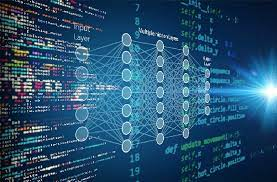
\includegraphics[width=3.33333in,height=\textheight]{images/clipboard-974366284.png}
\end{enumerate}

\begin{enumerate}
\def\labelenumi{\arabic{enumi}.}
\setcounter{enumi}{1}
\item
  Visualización y sus tres principios.

  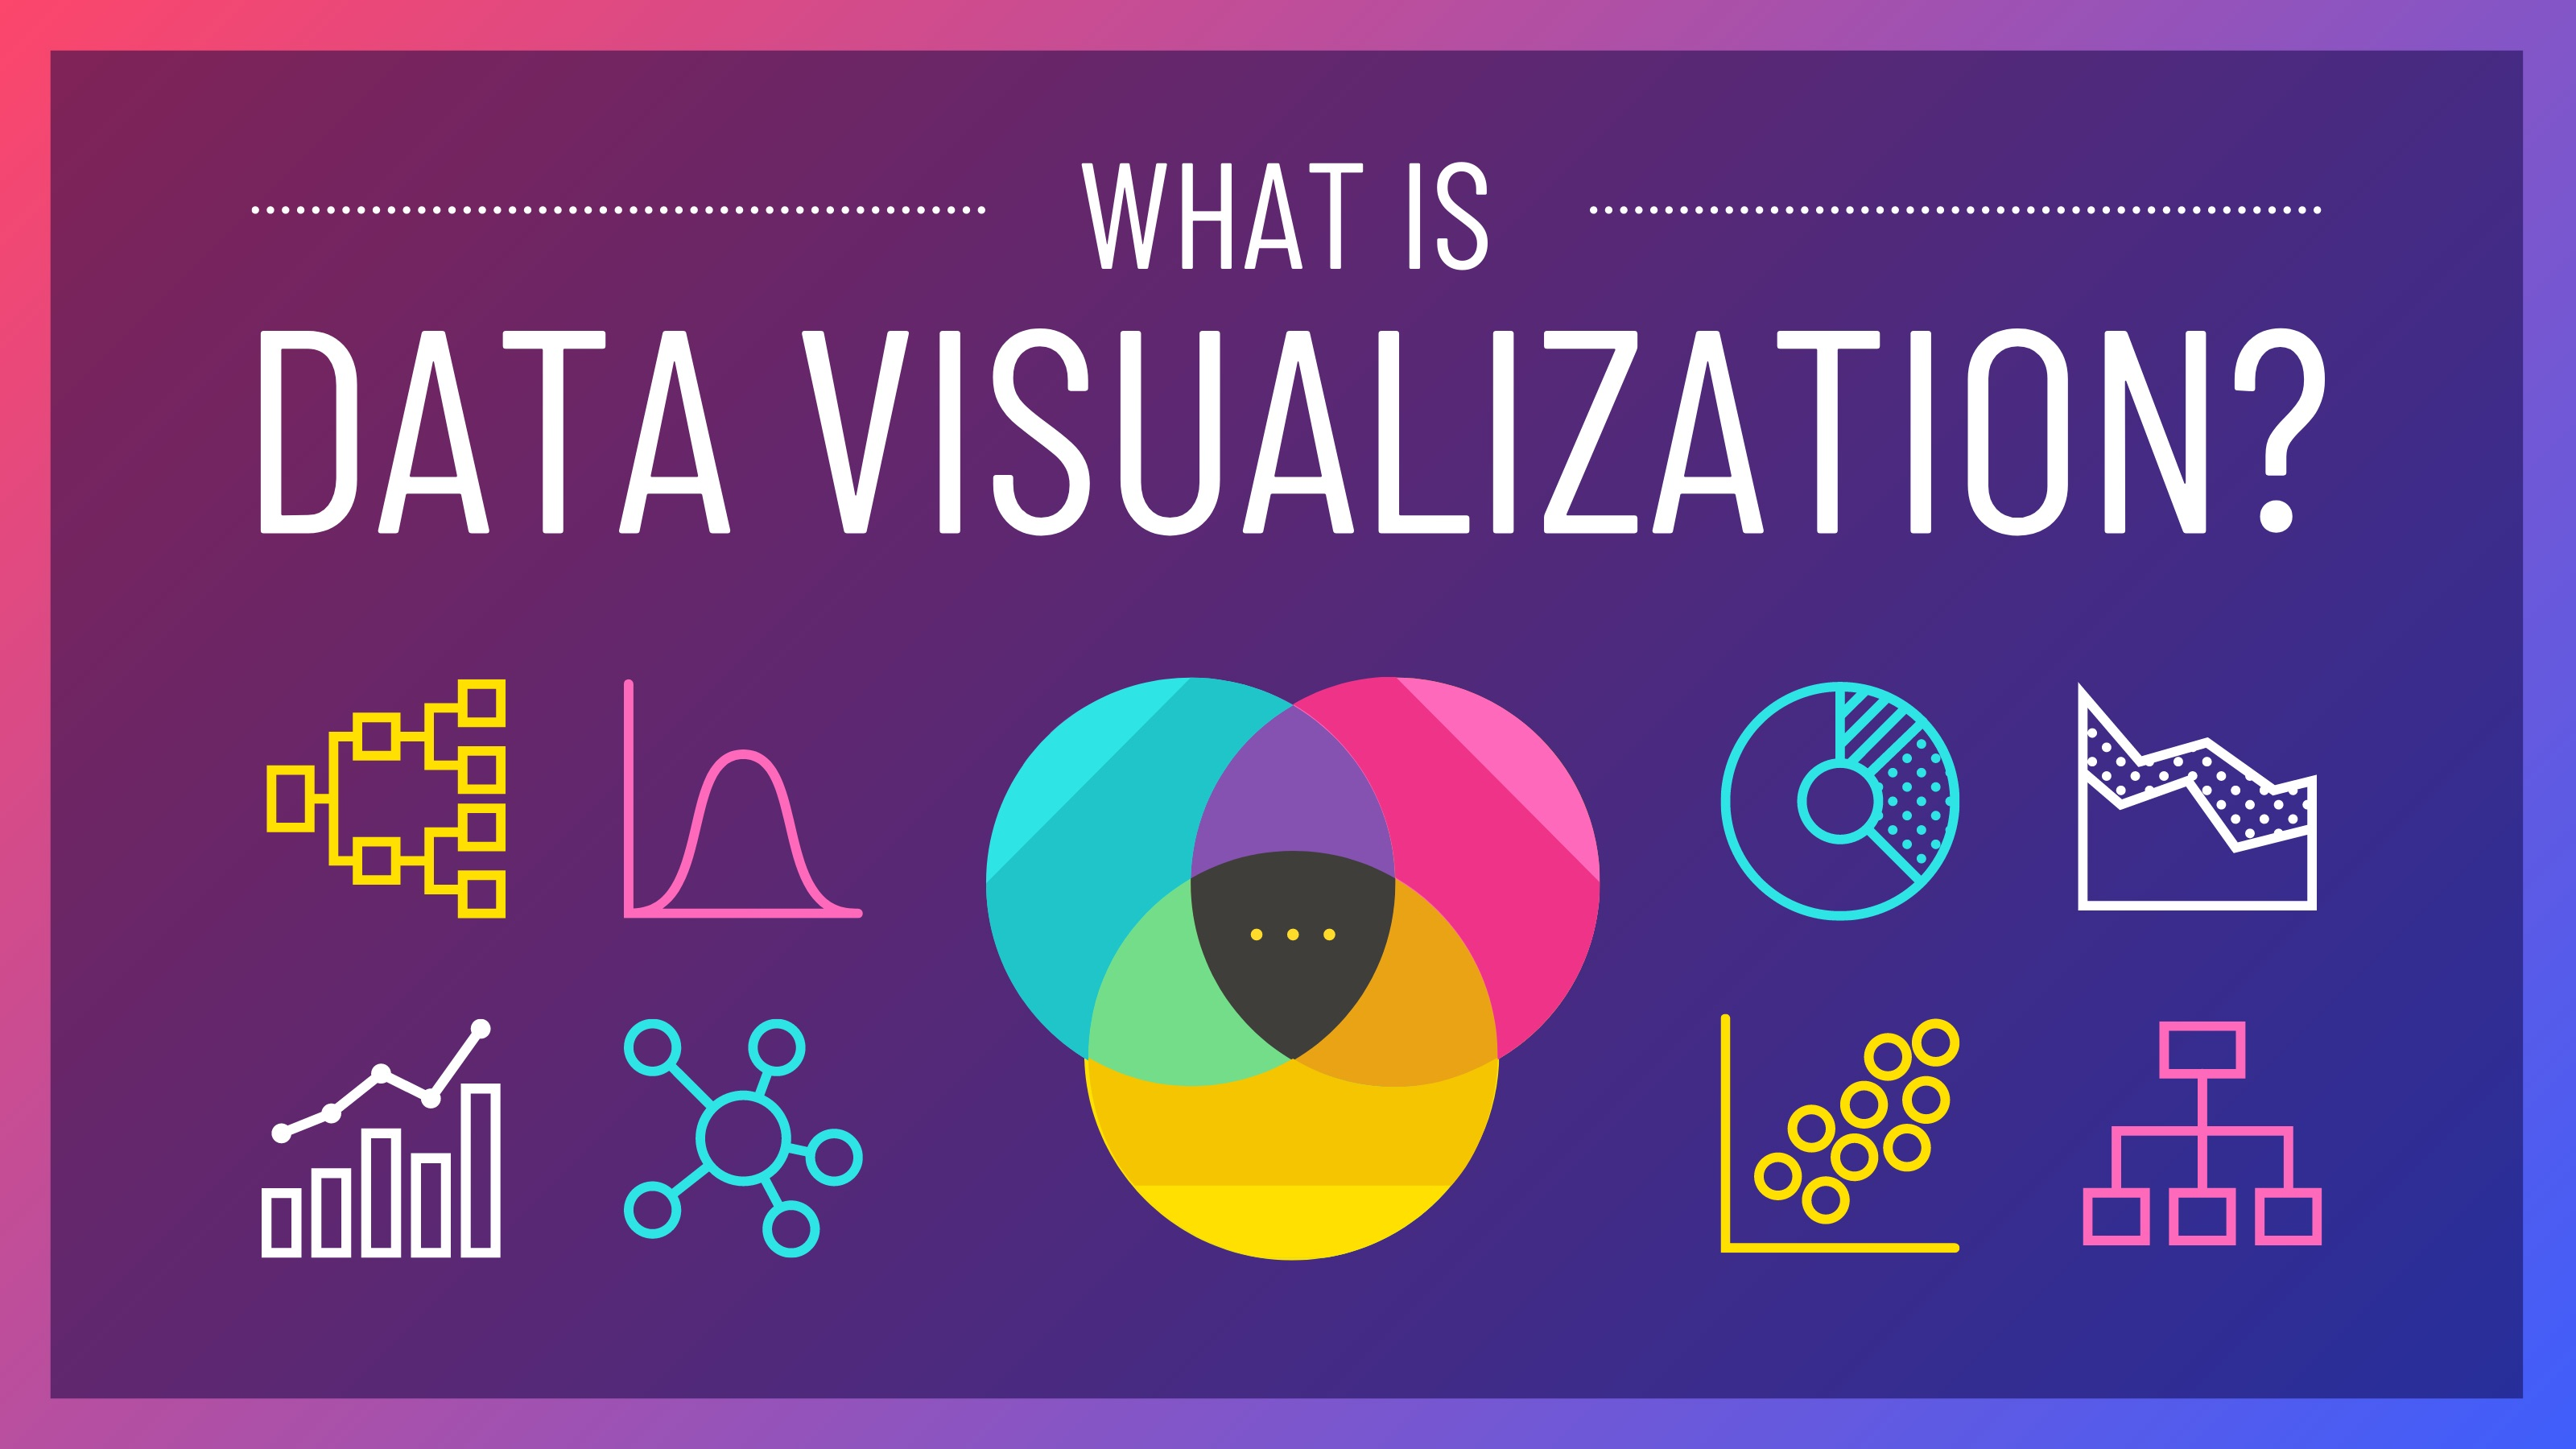
\includegraphics[width=3.59375in,height=\textheight]{images/clipboard-1163901538.png}
\end{enumerate}

\begin{enumerate}
\def\labelenumi{\arabic{enumi}.}
\setcounter{enumi}{2}
\tightlist
\item
  Actividad.
\end{enumerate}

\begin{figure}

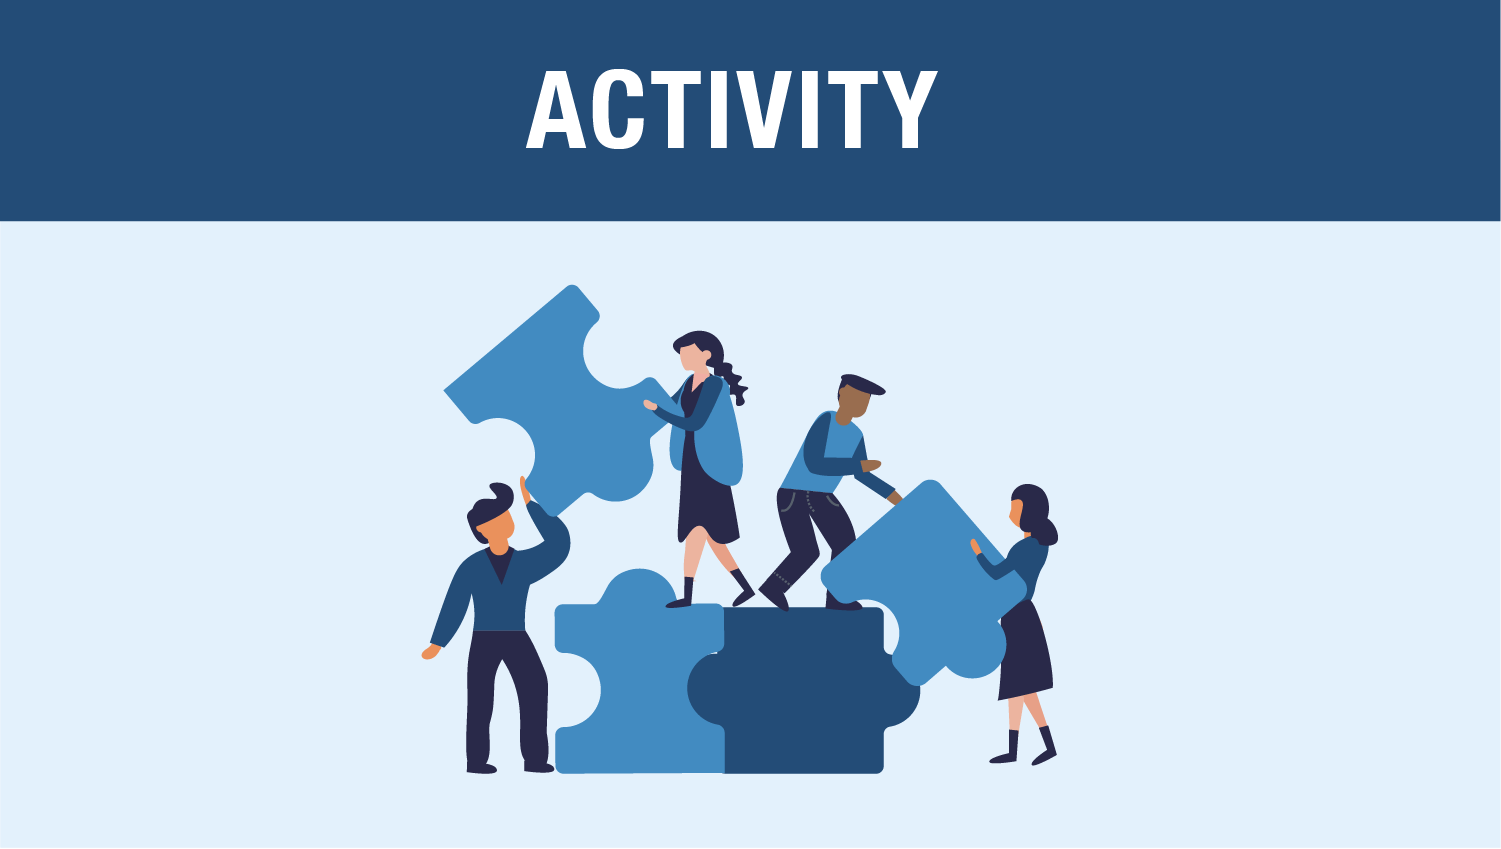
\includegraphics[width=3.55208in,height=\textheight]{images/clipboard-4224793803.png} \hfill{}

\end{figure}

\hypertarget{introducciuxf3n-a-ciencia-de-datos}{%
\section{Introducción a Ciencia de
Datos}\label{introducciuxf3n-a-ciencia-de-datos}}

\hypertarget{la-ciencia-de-datos-es}{%
\subsection{La ciencia de datos es
\ldots{}}\label{la-ciencia-de-datos-es}}

un campo interdisciplinario que utiliza métodos, procesos, algoritmos y
sistemas científicos para extraer conocimientos e ideas de muchos datos
estructurados y no estructurados.

. . .

\begin{figure}

{\centering 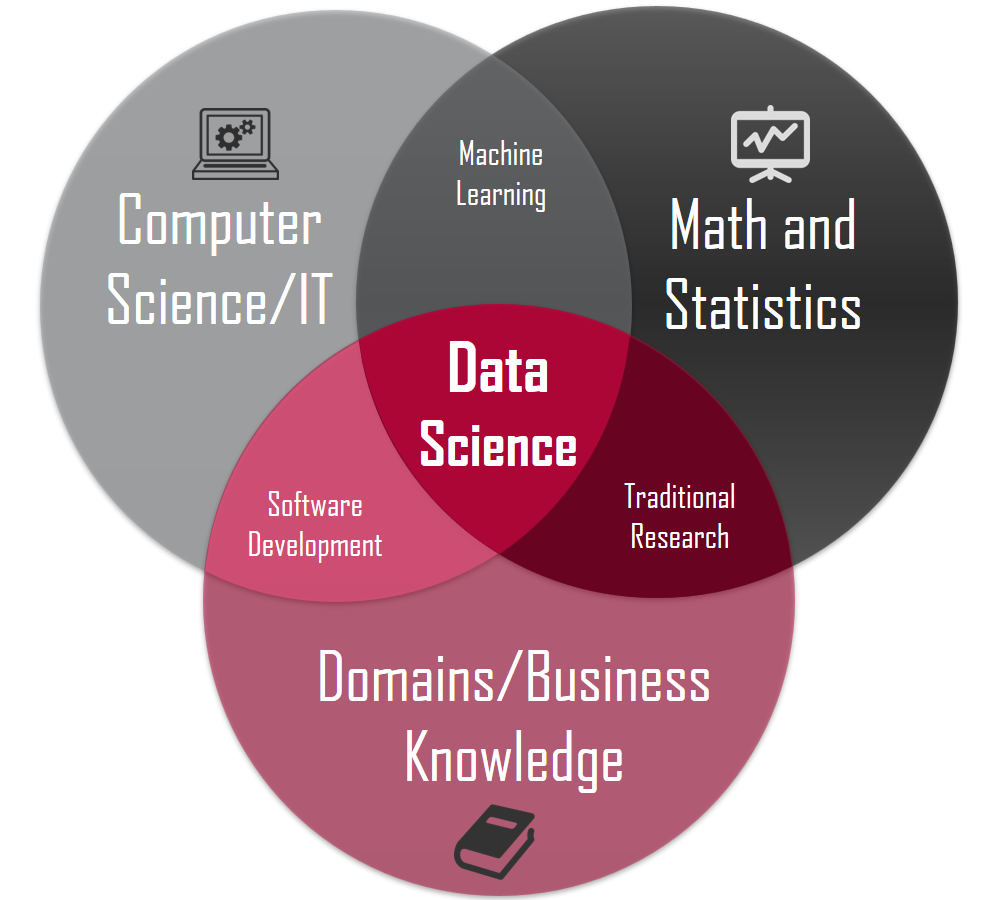
\includegraphics[width=3.92708in,height=\textheight]{images/clipboard-2707460623.png}

}

\end{figure}

\begin{figure}

{\centering 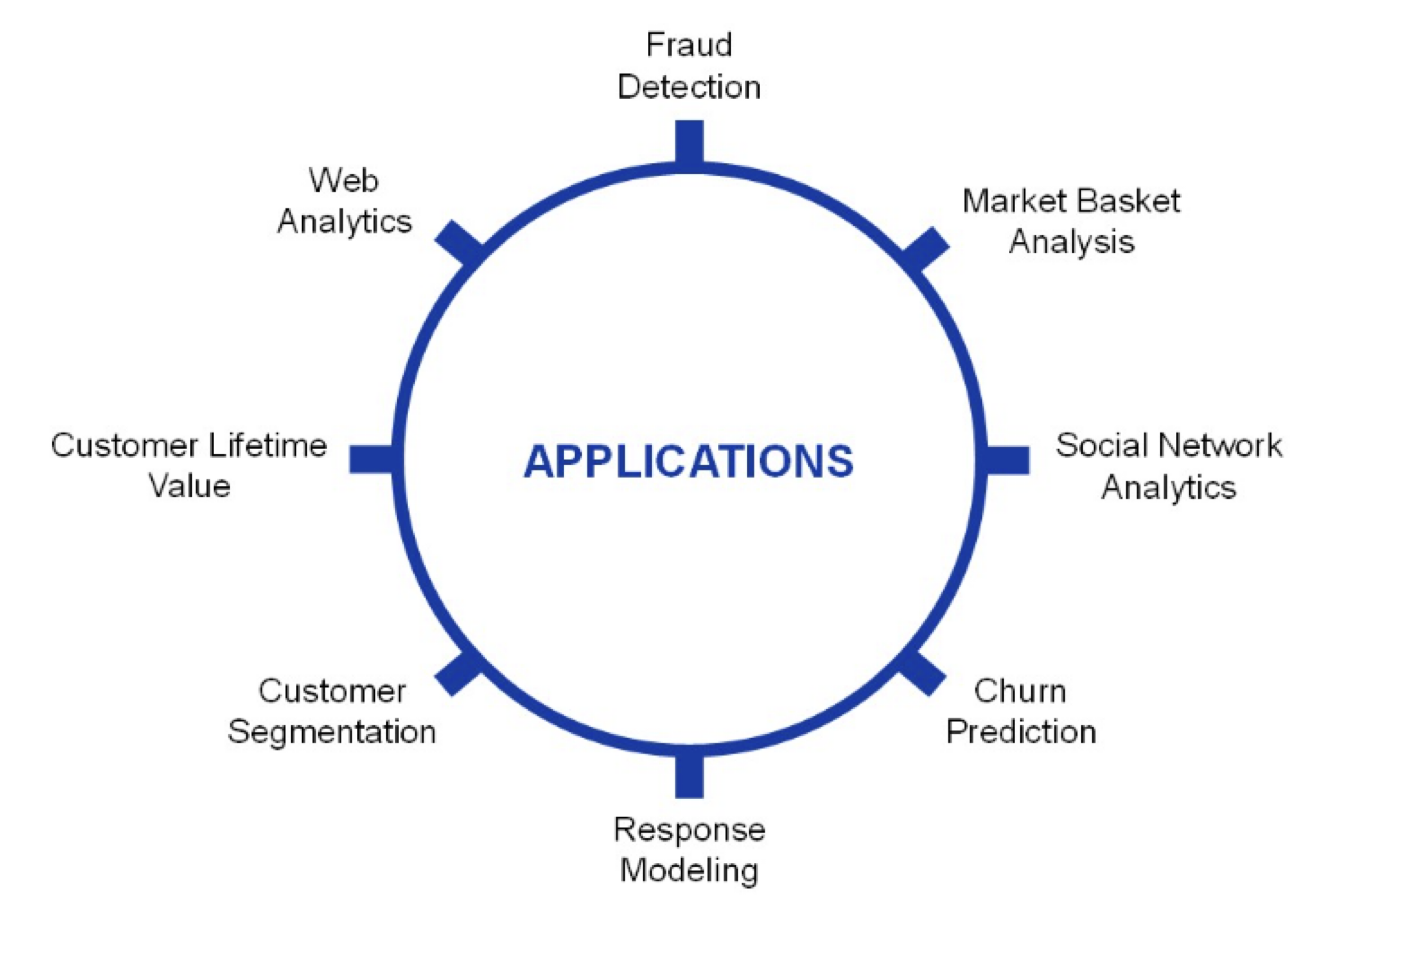
\includegraphics[width=5.05208in,height=\textheight]{images/clipboard-3242954590.png}

}

\end{figure}

\hypertarget{en-el-2004}{%
\subsection{En el 2004 \ldots{}}\label{en-el-2004}}

El huracán Frances estaba arrasando el Caribe y amenazando con golpear
directamente la costa atlántica de Florida.

. . .

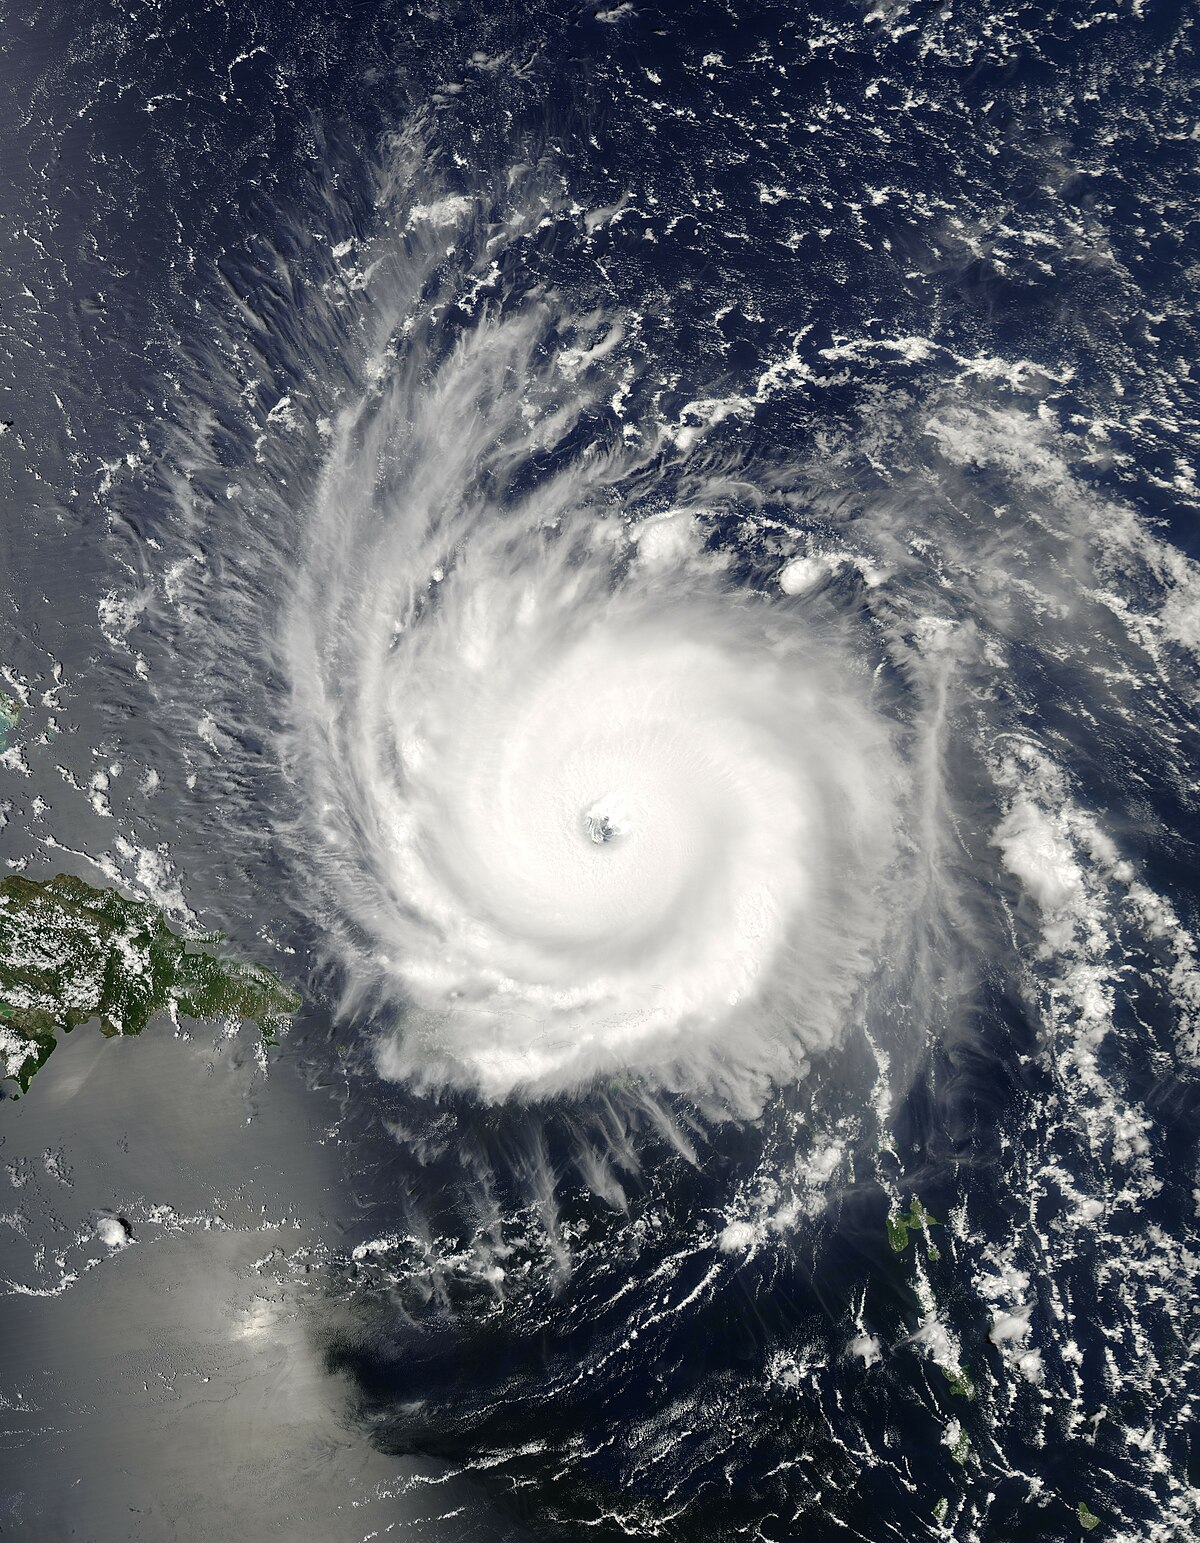
\includegraphics[width=2.02083in,height=\textheight]{images/clipboard-123225538.png}

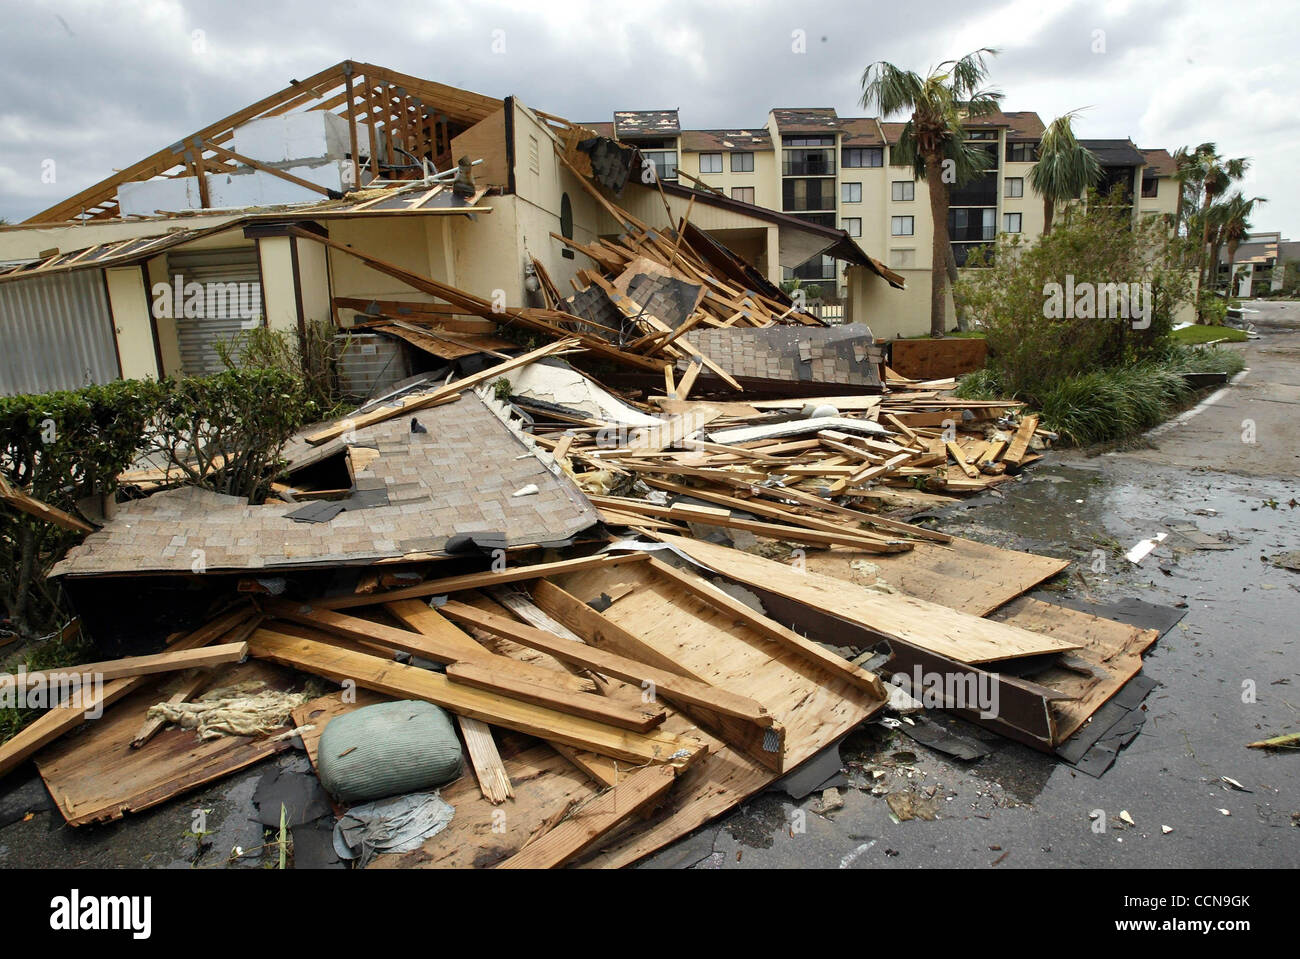
\includegraphics[width=2.79167in,height=\textheight]{Introduccion_files/mediabag/ft-pierce-9-6-04-un-.jpg}

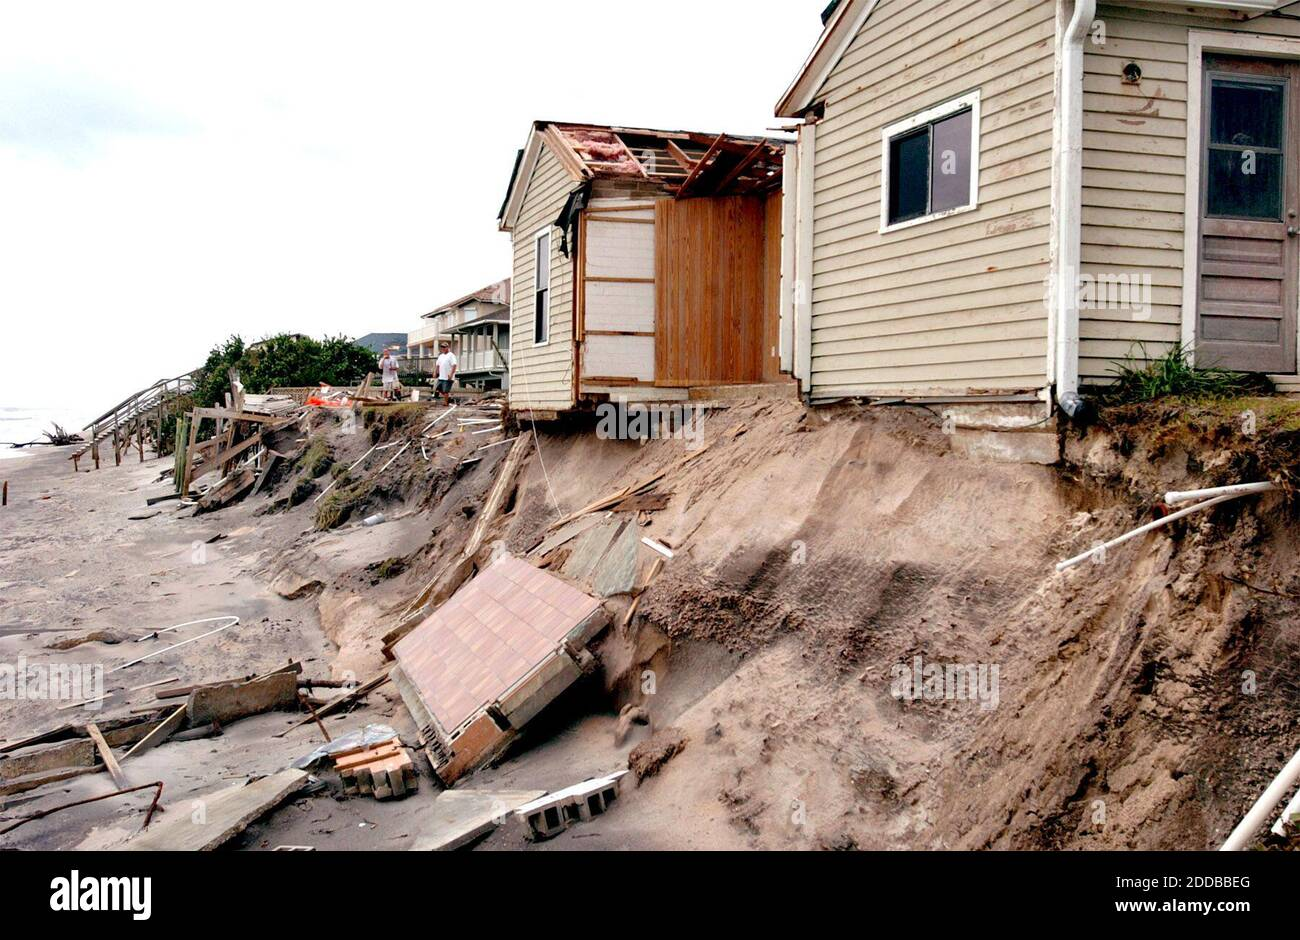
\includegraphics[width=2.91667in,height=\textheight]{images/clipboard-679480994.png}

. . .

Los residentes se dirigieron a terrenos más altos, pero en Arkansas, los
ejecutivos de Wal-Mart vieron que la situación ofrecía una gran
oportunidad para una de sus armas más nuevas basadas en datos:
\textbf{\emph{la tecnología predictiva}}.

\hypertarget{section}{%
\subsection{}\label{section}}

Una semana antes de que la tormenta tocara tierra, Linda M. Dillman,
directora de información de Wal-Mart, presionó a su personal para que
elaboraran pronósticos basados en lo que había sucedido cuando el
huracán Charley azotó varias semanas antes.

Respaldada por billones de bytes de historial de compradores almacenados
en el almacén de datos de Wal-Mart, consideró que la empresa podría
``empezar a predecir lo que va a suceder, en lugar de esperar a que
suceda'', como ella dijo.

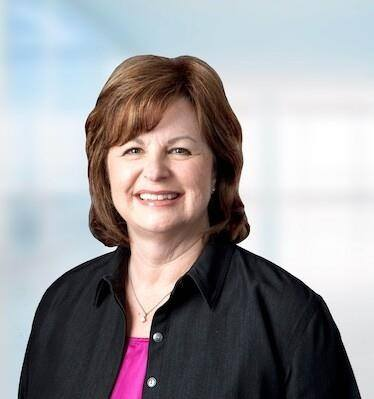
\includegraphics[width=2.33333in,height=\textheight]{images/clipboard-3960378011.png}


\includegraphics[width=5.375in,height=\textheight]{images/clipboard-4213549697.png}

\hypertarget{de-hecho-eso-es-lo-que-pasuxf3}{%
\subsection{¡De hecho, eso es lo que
pasó!}\label{de-hecho-eso-es-lo-que-pasuxf3}}

El New York Times informó

\begin{quote}
\emph{``\ldots{} los expertos analizaron los datos y descubrieron que
las tiendas efectivamente necesitarían ciertos productos, y no sólo las
habituales linternas.}''
\end{quote}

Dillman dijo

\begin{quote}
\emph{``No sabíamos en el pasado que las Pop-Tarts de fresa aumentan sus
ventas, como siete veces su tasa de ventas normal, antes de un
huracán''}
\end{quote}

\begin{figure}

{\centering 

\href{https://www.nytimes.com/2004/11/14/business/yourmoney/what-walmart-knows-about-customers-habits.html}{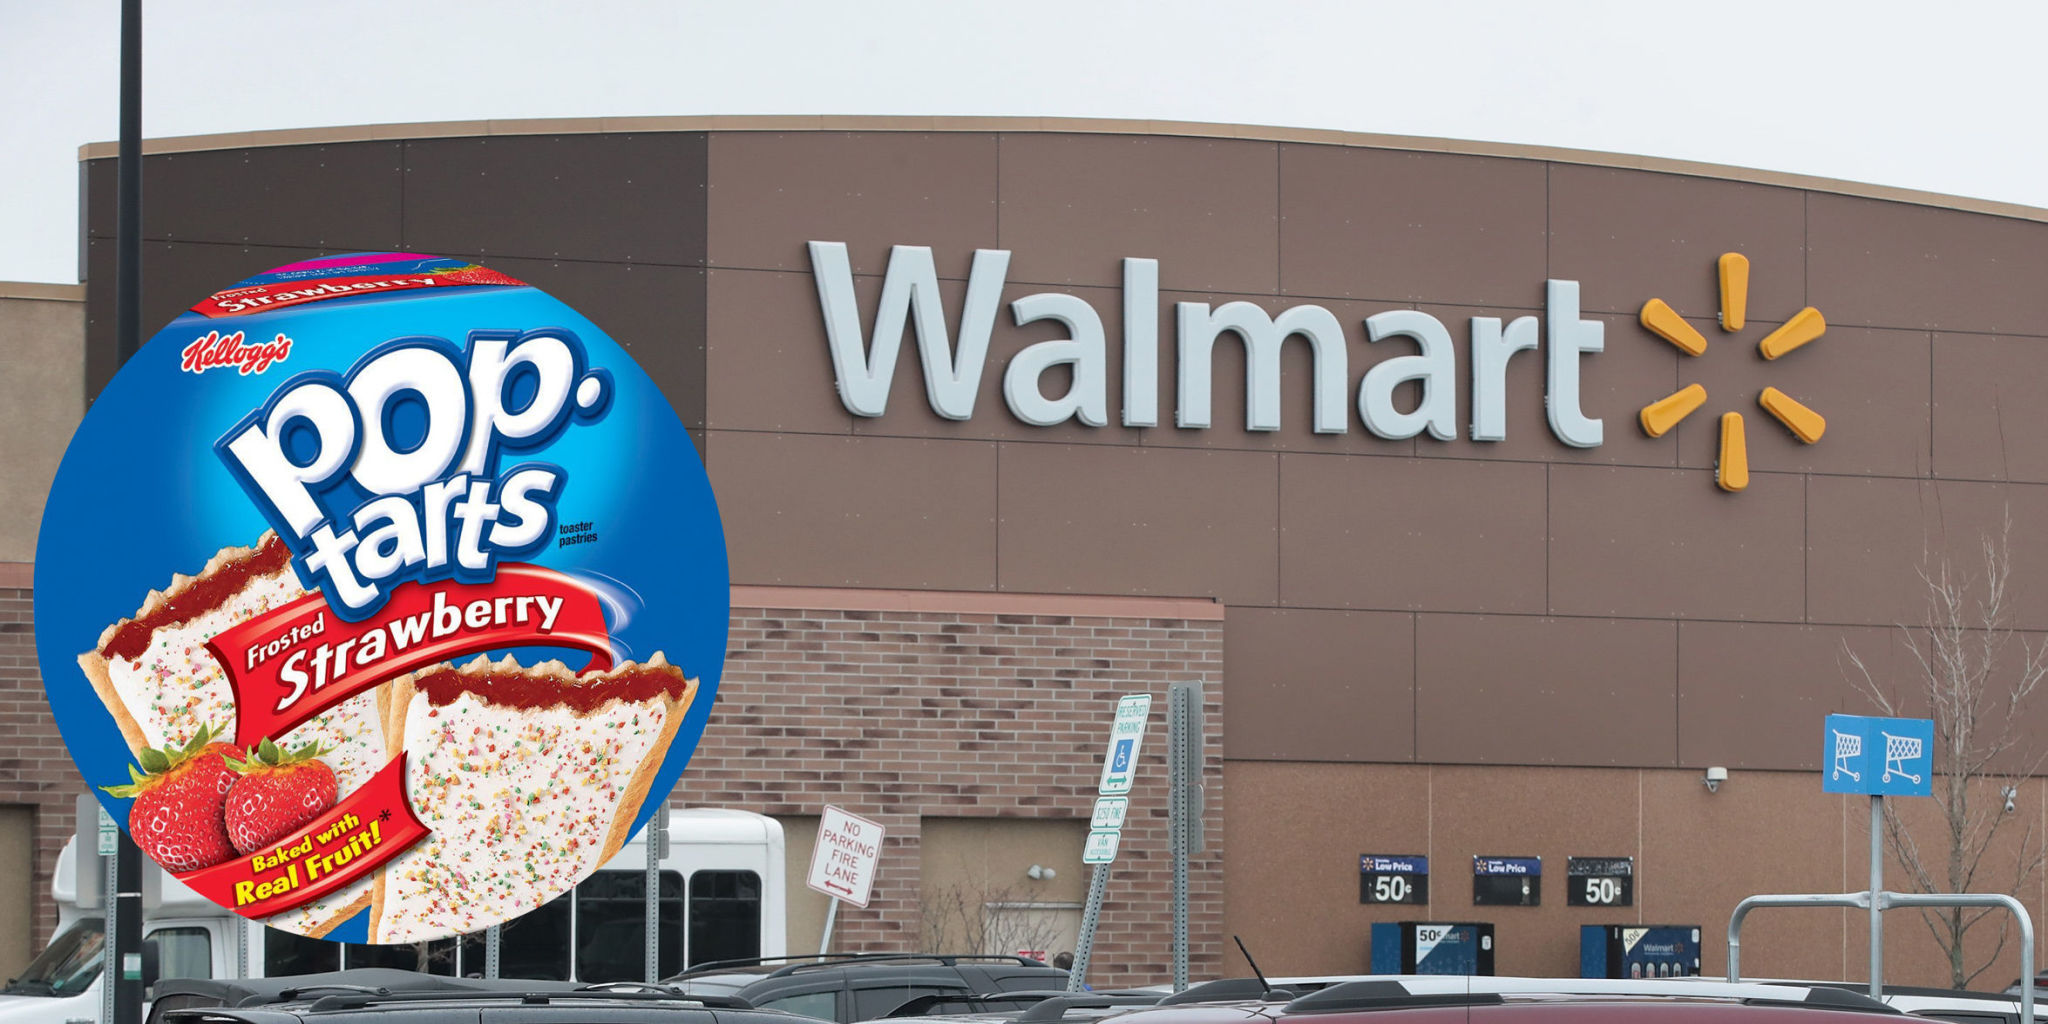
\includegraphics[width=5.51042in,height=\textheight]{images/clipboard-3670330051.png}}

}

\end{figure}

\hypertarget{el-esquema-de-ciencia-de-datos}{%
\subsection{El esquema de ciencia de
datos}\label{el-esquema-de-ciencia-de-datos}}

\begin{figure}

{\centering 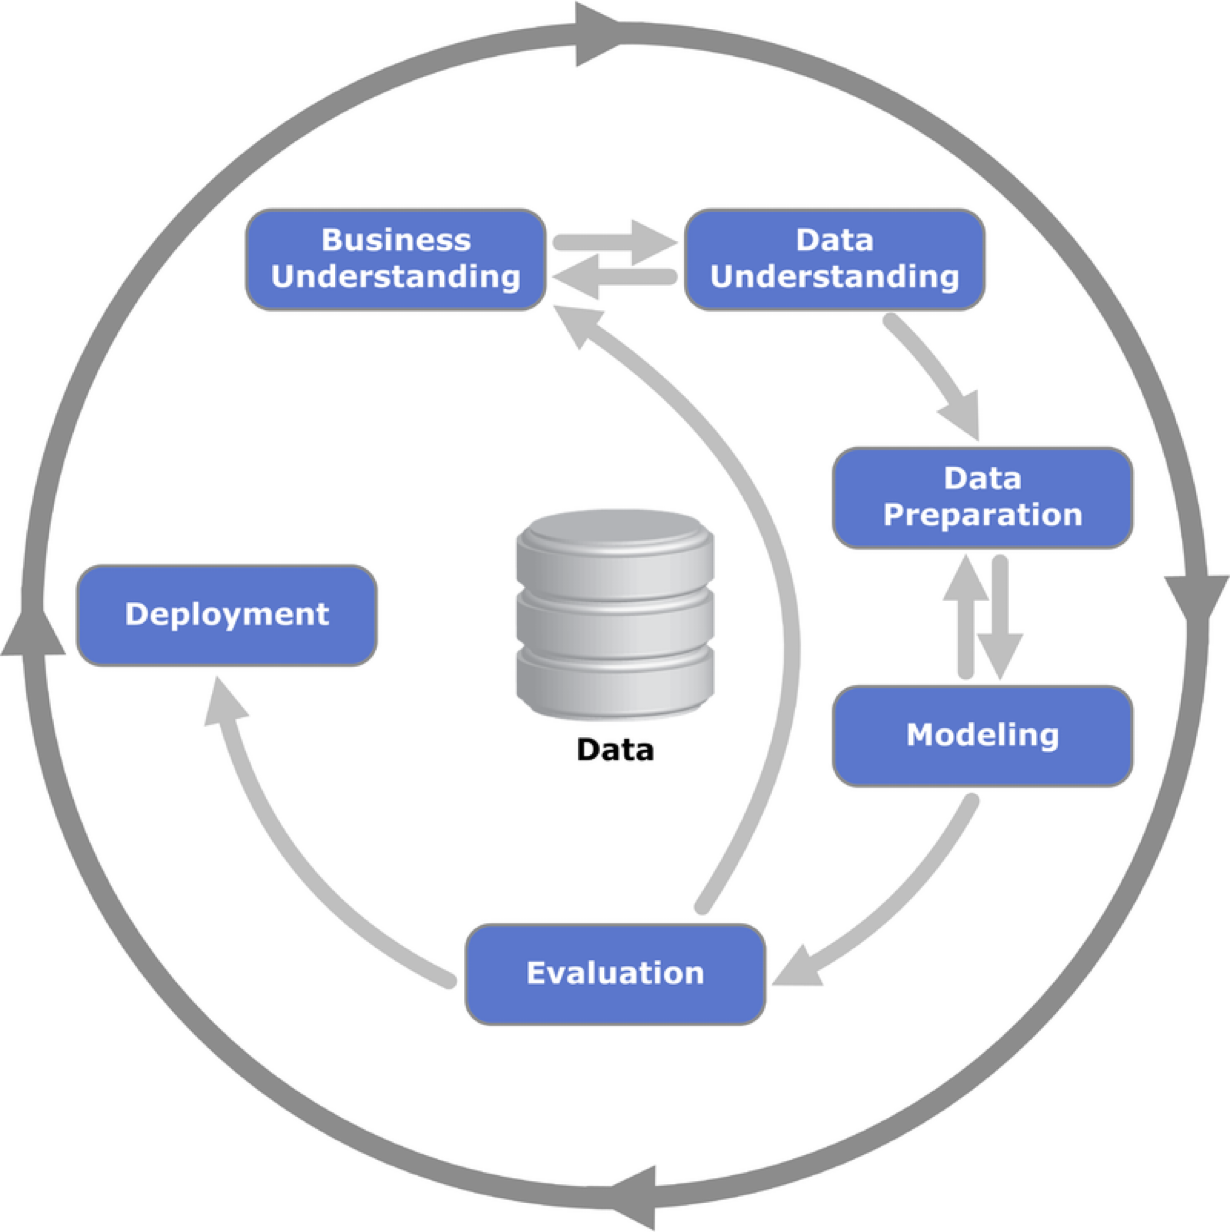
\includegraphics{images/clipboard-4096324521.png}

}

\end{figure}

\hypertarget{business-understanding}{%
\subsection{Business understanding}\label{business-understanding}}

\begin{itemize}
\item
  La comprensión empresarial se refiere a definir el problema
  empresarial a resolver.
\item
  El objetivo es reformular el problema empresarial como un problema de
  ciencia de datos.
\item
  A menudo, reformular el problema y diseñar una solución es un proceso
  iterativo.
\end{itemize}

\hypertarget{data-understanding}{%
\subsection{Data understanding}\label{data-understanding}}

\begin{itemize}
\item
  Si el objetivo es resolver un problema empresarial, los datos que
  componen la materia prima disponible a partir de la cual se construirá
  la solución.
\item
  Los datos disponibles rara vez coinciden con el problema.
\item
  Por ejemplo, los datos históricos a menudo se recopilan con fines no
  relacionados con el problema empresarial actual o sin ningún propósito
  explícito.
\end{itemize}

. . .

\begin{quote}
Nuestro objetivo es convertir los datos en información que contesten
preguntas útiles.
\end{quote}

\hypertarget{tipos-de-datos}{%
\subsection{Tipos de datos}\label{tipos-de-datos}}

{\textbf{Texto}}

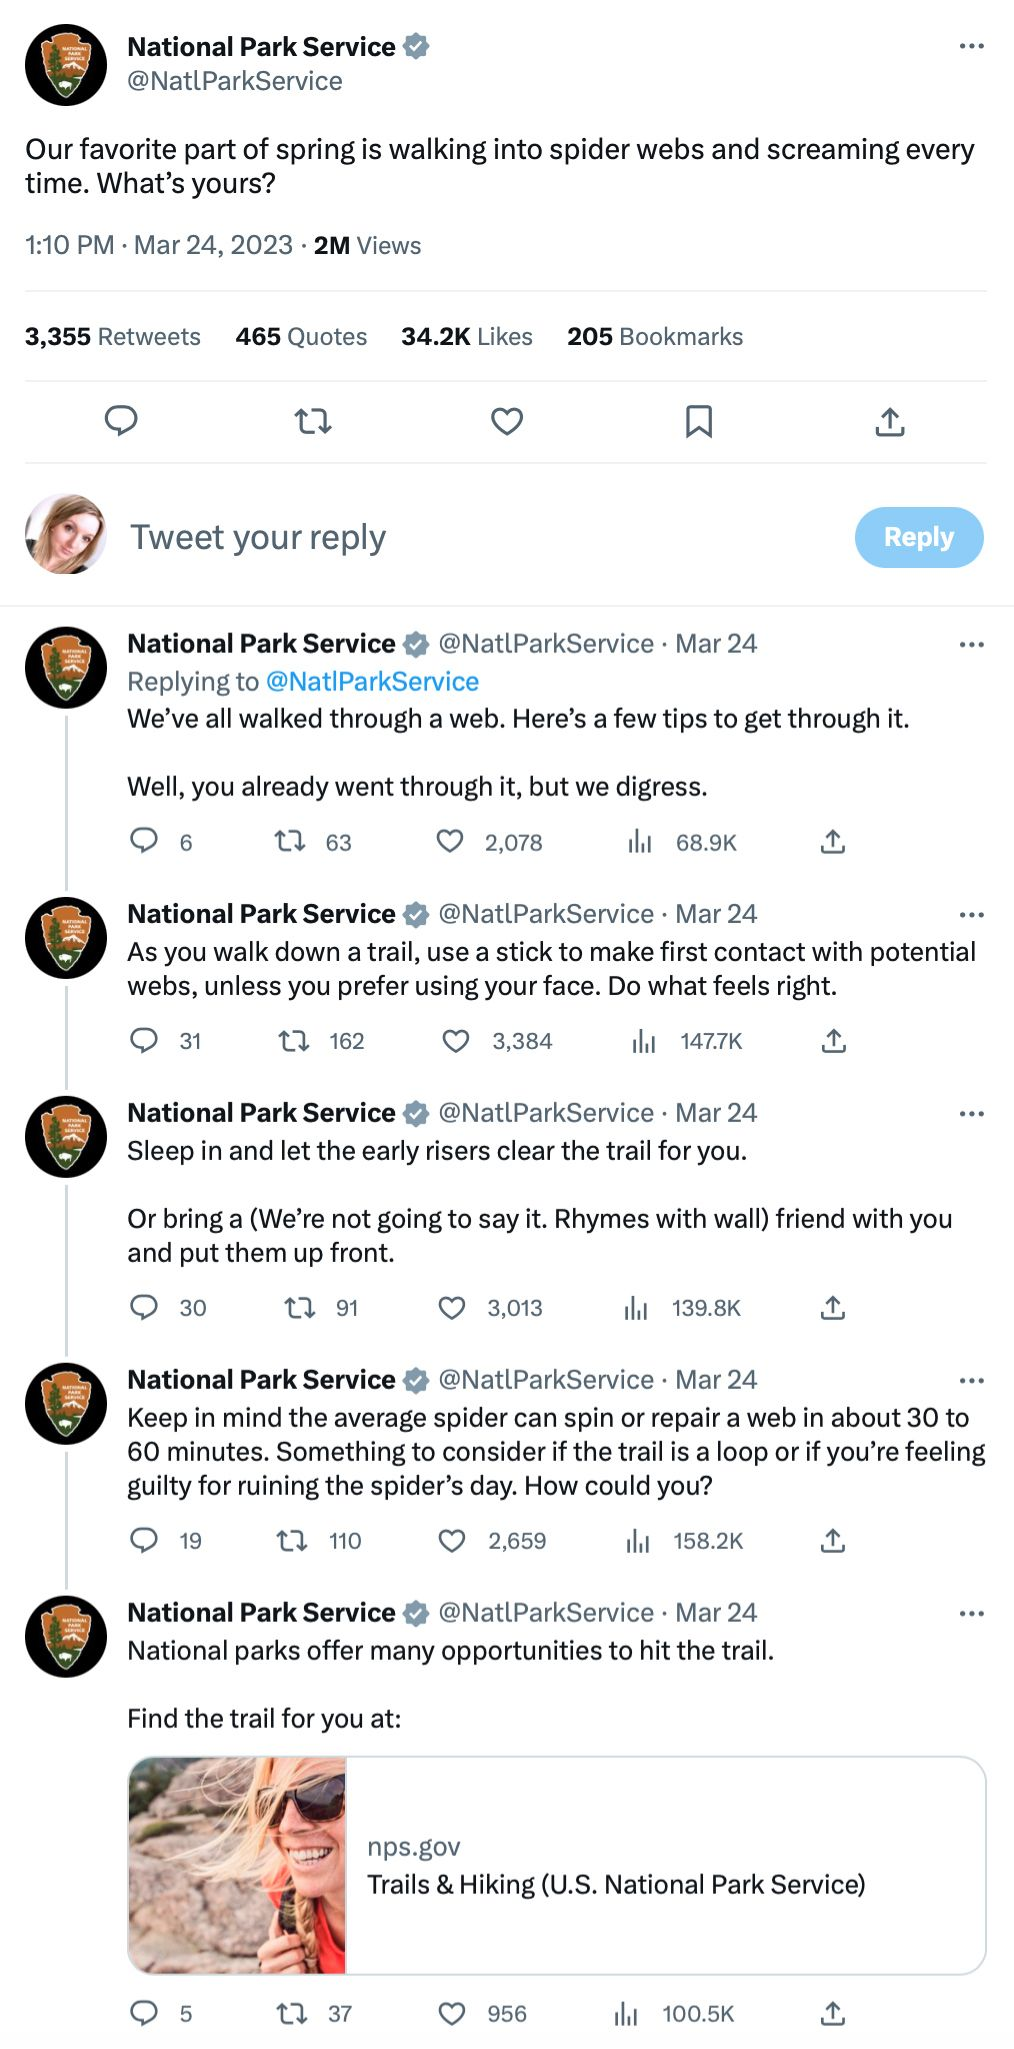
\includegraphics[width=5.32292in,height=\textheight]{images/clipboard-4167942809.png}

{\textbf{Imágenes}}

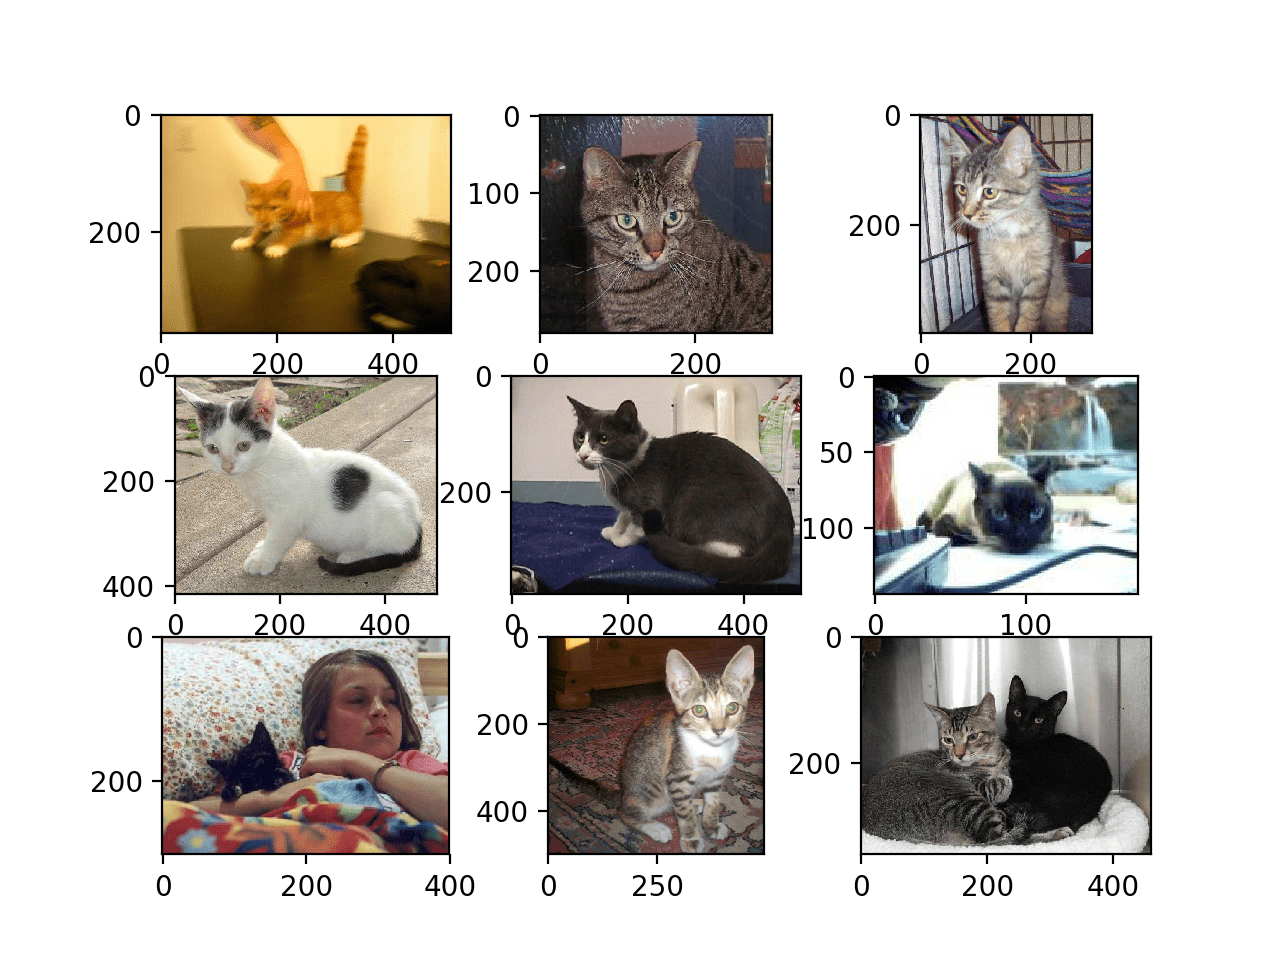
\includegraphics[width=5.48958in,height=\textheight]{images/clipboard-3296722573.png}

{\textbf{Video}}

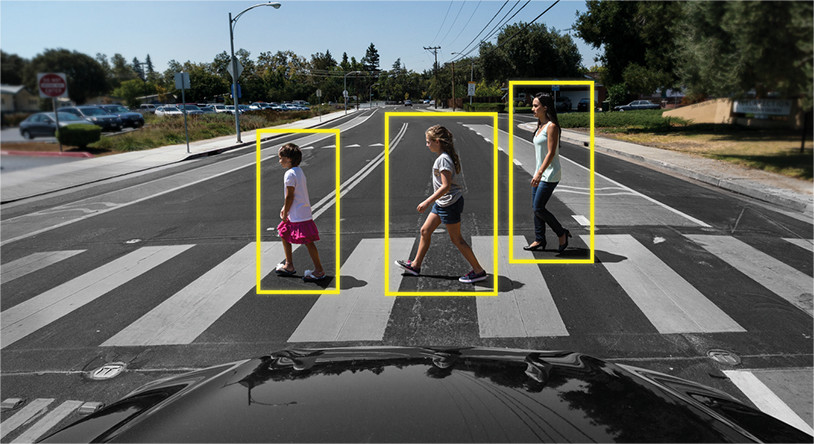
\includegraphics[width=4.17708in,height=\textheight]{images/clipboard-2123600827.png}

{\textbf{Audio}}

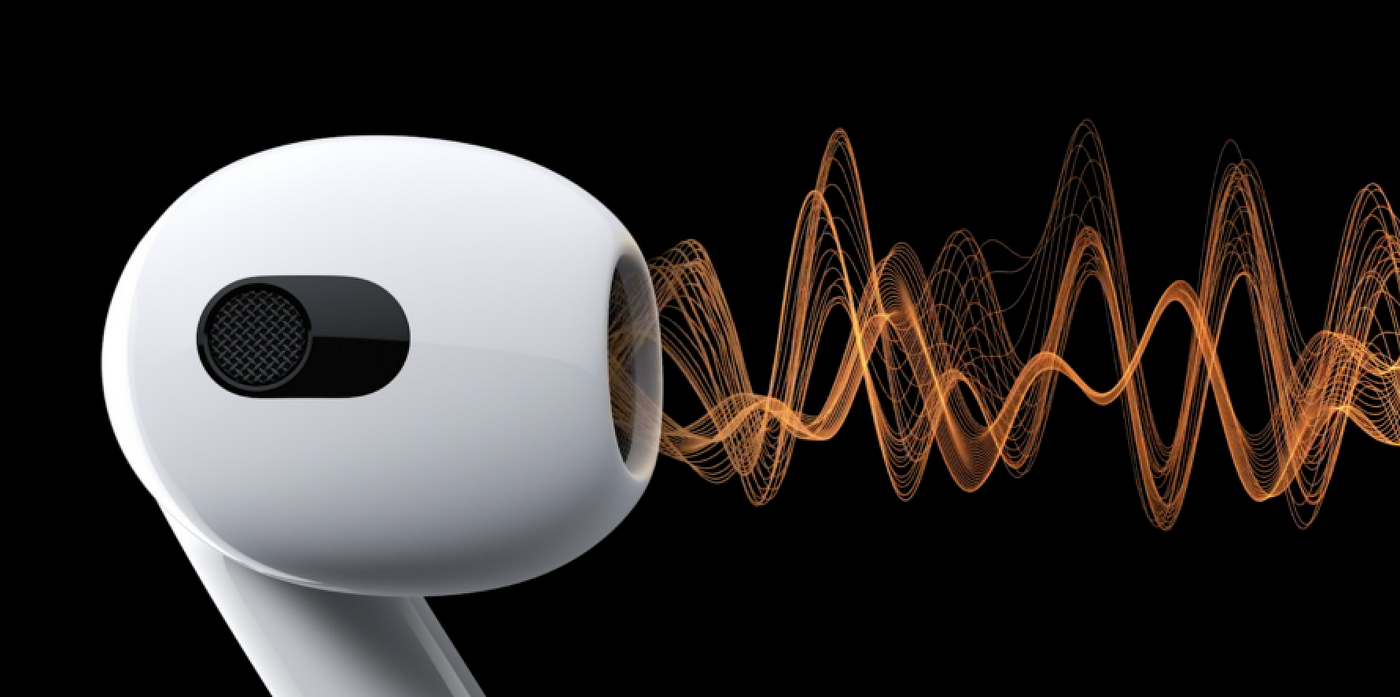
\includegraphics{images/clipboard-2206237365.png}

\hypertarget{datos-nuxfamericos}{%
\subsection{Datos númericos}\label{datos-nuxfamericos}}

La metodología de ciencia de datos esta basada en datos númericos dados
en tablas.

\begin{figure}

{\centering 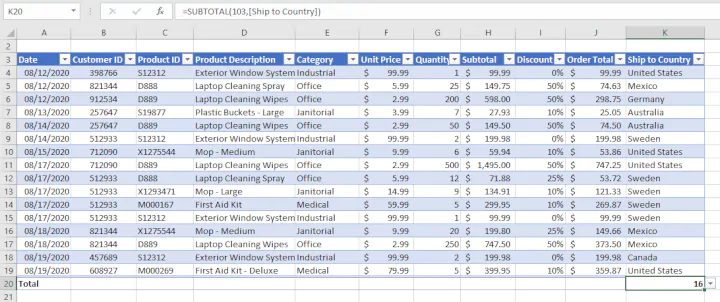
\includegraphics{images/9a292b70-64d7-475e-9ffa-22c019609752_lossy.png}

}

\end{figure}

\begin{quote}
De hecho, los textos, imágenes, videos o audios son transformados a este
formato para procesarlos.
\end{quote}

. . .

{\textbf{\emph{En este curso, asumiremos que los datos están en una
tabla.}}}

Mas importante, asumiremos que los datos han sido limpiados y no
contienen typos o observaciones extrañas.

\hypertarget{la-situaciuxf3n-problema}{%
\subsection{La Situación Problema}\label{la-situaciuxf3n-problema}}

YouTube es una plataforma para compartir vídeos ampliamente conocida por
la diversidad de vídeos subidos por sus usuarios.

El sitio permite a sus usuarios cargar, ver, calificar, compartir y
comentar videos.

Un tipo particular de usuario es el \emph{creador de contenido}, quien
frecuentemente crea y sube videos entretenidos a la plataforma.

\begin{figure}

\hfill{} 
\includegraphics[width=4.55208in,height=\textheight]{images/clipboard-2009057073.png}

\end{figure}

\hypertarget{objetivo-de-la-situaciuxf3n-problema}{%
\subsection{Objetivo de la situación
problema}\label{objetivo-de-la-situaciuxf3n-problema}}

\begin{quote}
Esta situación problema concierne la creación de un póster que informe a
un creador de contenido de Youtube los aspectos mas importantes del
formato miniatura de un video. Es decir, que estén asociadas a un número
de vistas grande.
\end{quote}

Para esto, tendrás a tu disposición una base de datos con 7242 videos y
51 variables que se encuentra en el archivo ``YouTube\_Dataset.xlsx.''

Puedes encontrar más información en nuestra página de Canvas.

\hypertarget{visualizaciuxf3n-de-datos-y-sus-principios}{%
\section{Visualización de datos y sus
principios}\label{visualizaciuxf3n-de-datos-y-sus-principios}}

\hypertarget{quuxe9-es-la-visualizaciuxf3n-de-datos}{%
\subsection{¿Qué es la visualización de
datos?}\label{quuxe9-es-la-visualizaciuxf3n-de-datos}}

\begin{quote}
``Una visualización {[}de datos{]} es cualquier presentación visual
destinada a revelar evidencia, haciendo visible lo invisible'' Alberto
Cairo (2015).
\end{quote}

\begin{figure}

{\centering 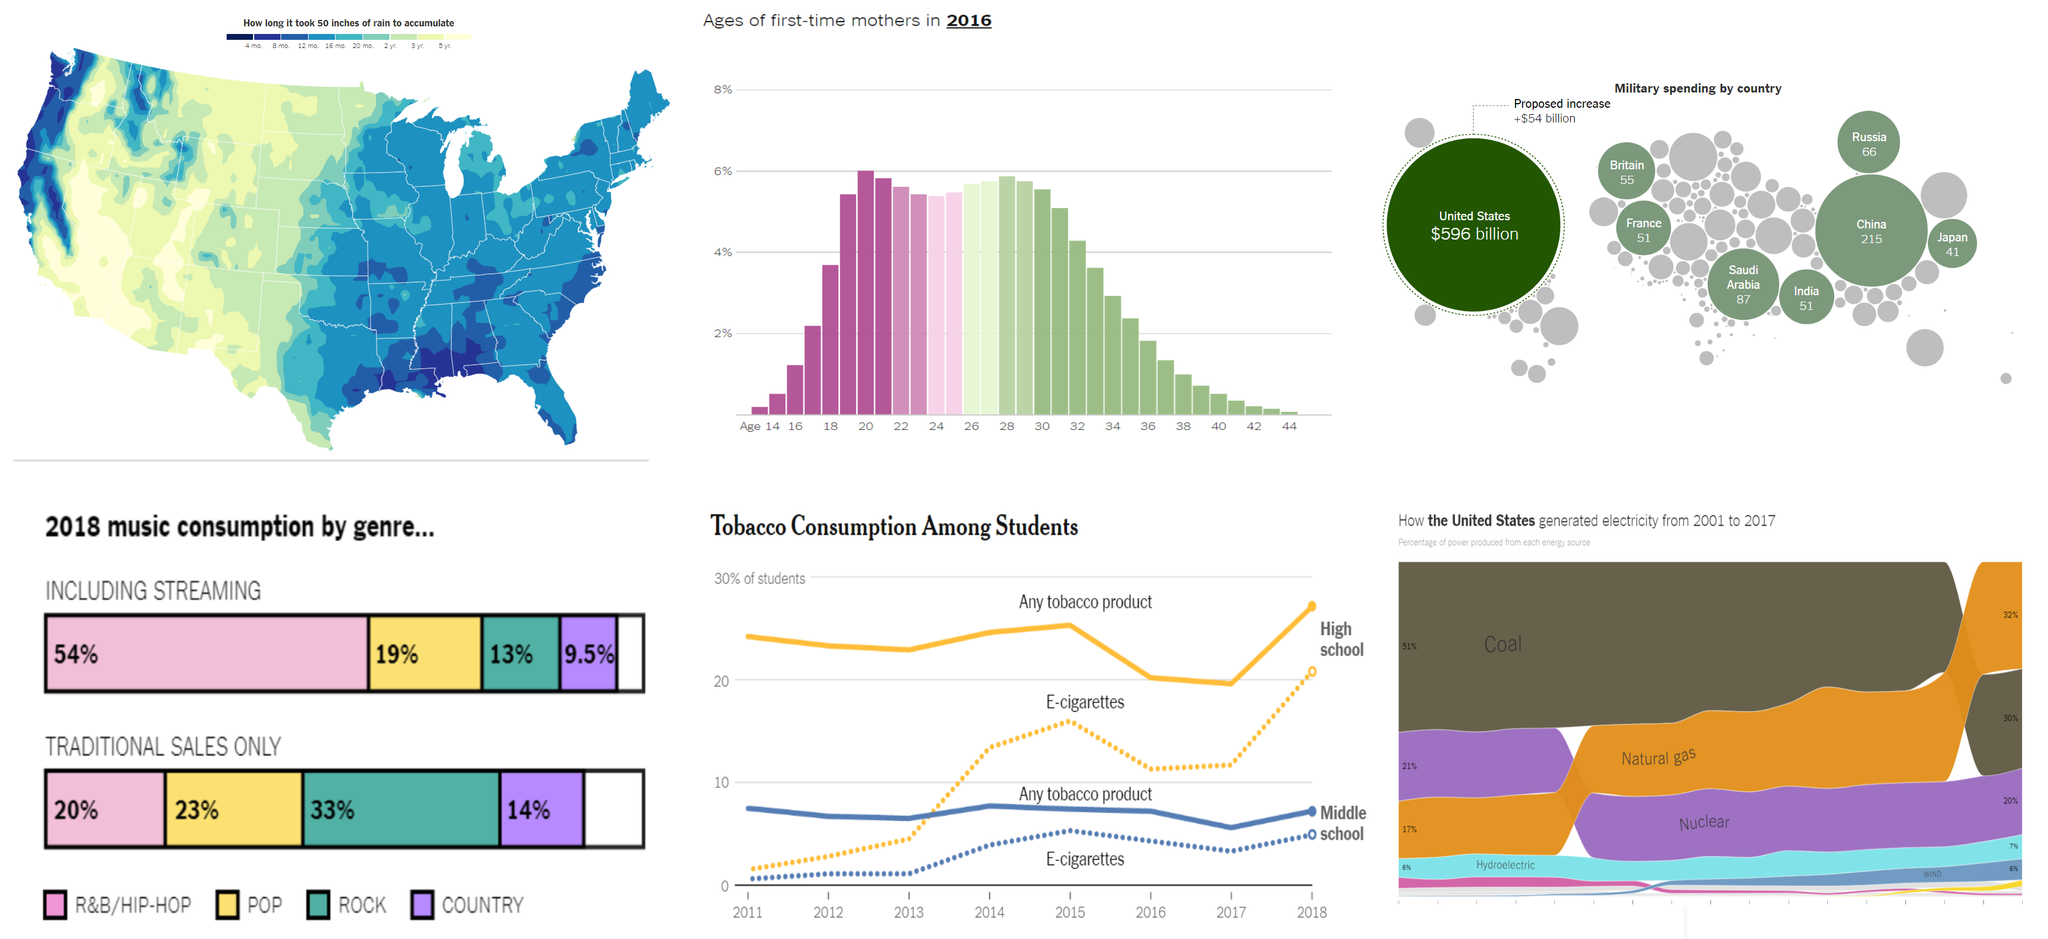
\includegraphics[width=8.47917in,height=\textheight]{images/clipboard-3803538817.png}

}

\end{figure}

\hypertarget{section-1}{%
\subsection{}\label{section-1}}

En escencia, una visualización de datos te permite profundizar en
conjuntos de datos complejos para obtener información significativa
mediante el uso de pantallas gráficas.

Las visualizaciones de datos se ocupan principalmente de proporcionar
evidencia y permitir que la audiencia explore y llegue a sus propias
conclusiones sobre lo que las visualizaciones revelan sobre los datos.

As data scientists, we create data visualizations in order to understand
our data and explain our analyses to other people. A plot should have a
message, and it's our job to communicate this message as clearly as
possible.

\hypertarget{los-3-principios-de-la-visualizaciuxf3n-de-datos}{%
\section{Los 3 principios de la visualización de
datos}\label{los-3-principios-de-la-visualizaciuxf3n-de-datos}}

\hypertarget{principio-1-formula-el-mensaje}{%
\subsection{\texorpdfstring{\textbf{\emph{Principio 1}:} Formula el
mensaje}{Principio 1: Formula el mensaje}}\label{principio-1-formula-el-mensaje}}

Muchas veces el mensaje se obtiene al contestar una pregunta de interés.


\includegraphics[width=5.19792in,height=\textheight]{images/clipboard-1758479249.png}

\begin{figure}

{\centering 

\href{https://www.google.com/url?sa=i\&url=https\%3A\%2F\%2Fwww.alamy.com\%2Fbe-ready-to-lose-all-your-money-on-bitcoin-fca-tells-consumers-financial-newspaper-headline-in-guardian-12-january-2021-great-britain-uk-europe-image399276404.html\&psig=AOvVaw1j_DY1hqJ8N6YDmcJrt7O4\&ust=1706894768727000\&source=images\&cd=vfe\&opi=89978449\&ved=0CBIQjRxqFwoTCNiE4-PUioQDFQAAAAAdAAAAABAD}{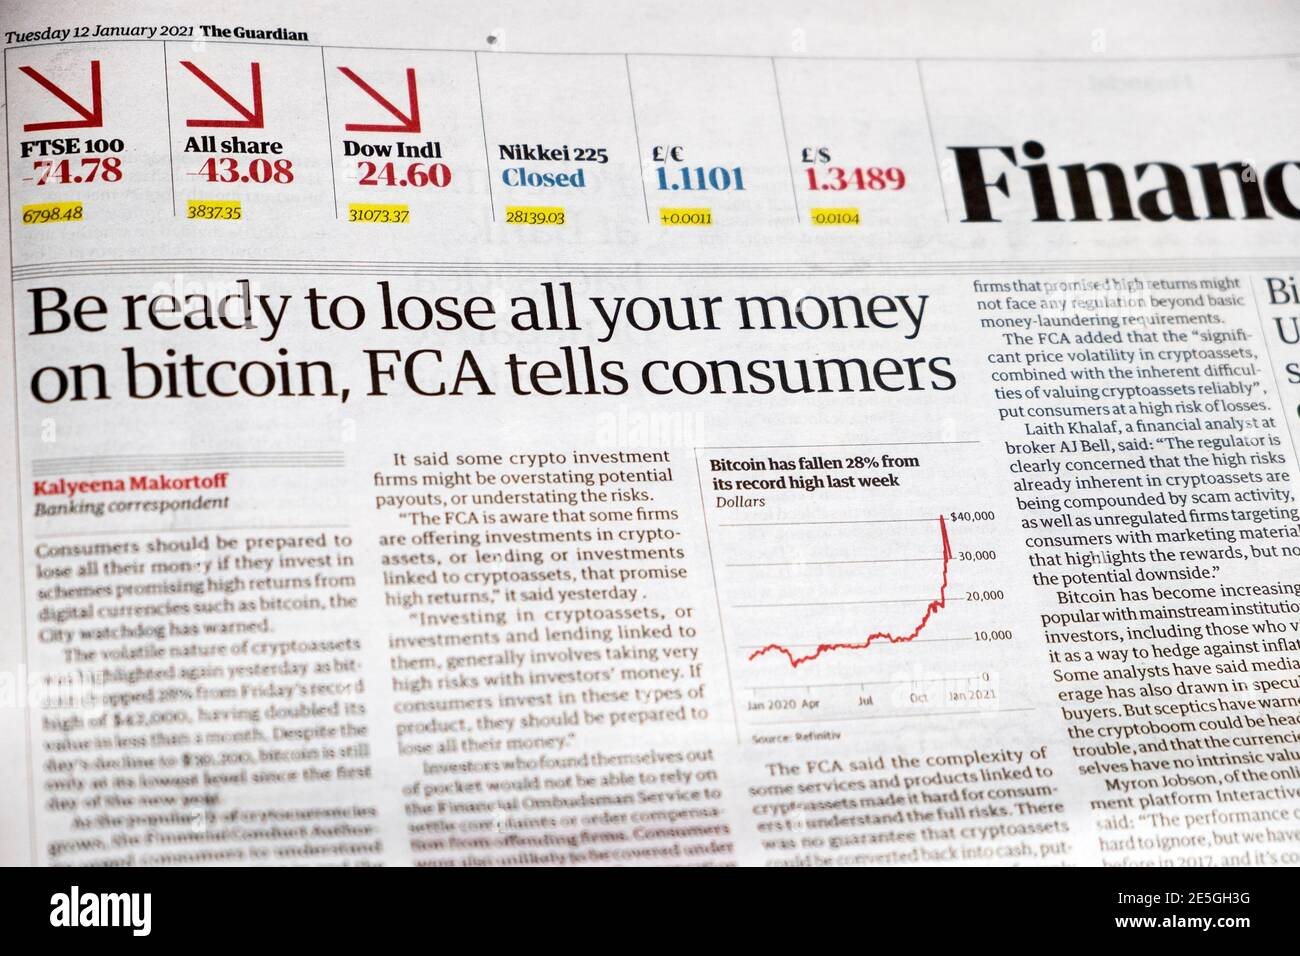
\includegraphics{Introduccion_files/mediabag/be-ready-to-lose-all.jpg}}

}

\end{figure}

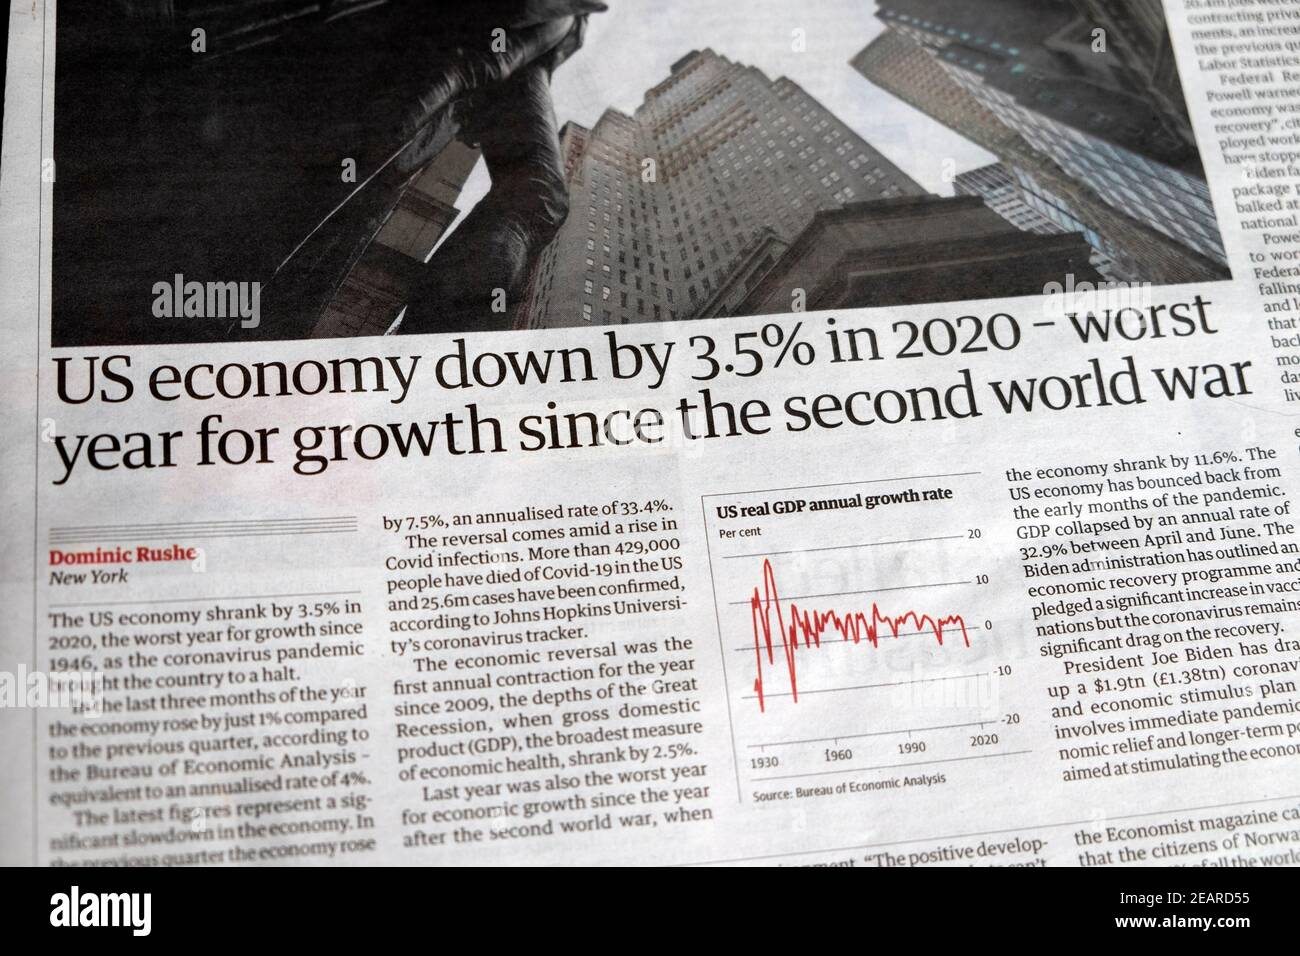
\includegraphics{images/clipboard-1023529598.png}

El mensaje puede ser una pregunta

\begin{itemize}
\item
  ¿Cuál es la comparación importante?
\item
  ¿Cómo la enfatizamos?
\item
  Do you have reason to expect that one group/observation might be
  different?
\item
  Why might your finding about shape matter?
\item
  What additional comparison might bring added value to the
  investigation?
\item
  Are there any potentially important features to create comparisons
  with/against?
\end{itemize}

{[}Incluir noticias del new york times{]}

\hypertarget{principio-2-transforma-los-datos-en-informaciuxf3n}{%
\subsection{\texorpdfstring{\textbf{\emph{Principio 2}: \emph{Transforma
los datos en
información}}}{Principio 2: Transforma los datos en información}}\label{principio-2-transforma-los-datos-en-informaciuxf3n}}

Tu gráfica debe de usar los datos para transmitir el mensaje o contestar
la pregunta. Es decir, debe de transformar los datos en información.

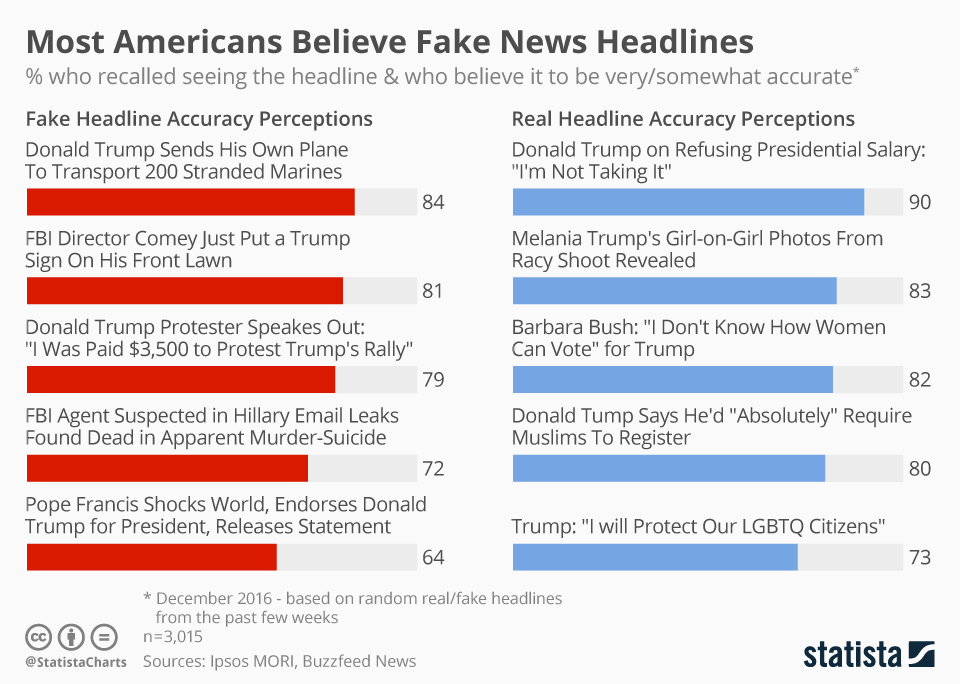
\includegraphics{images/clipboard-4189732703.png}

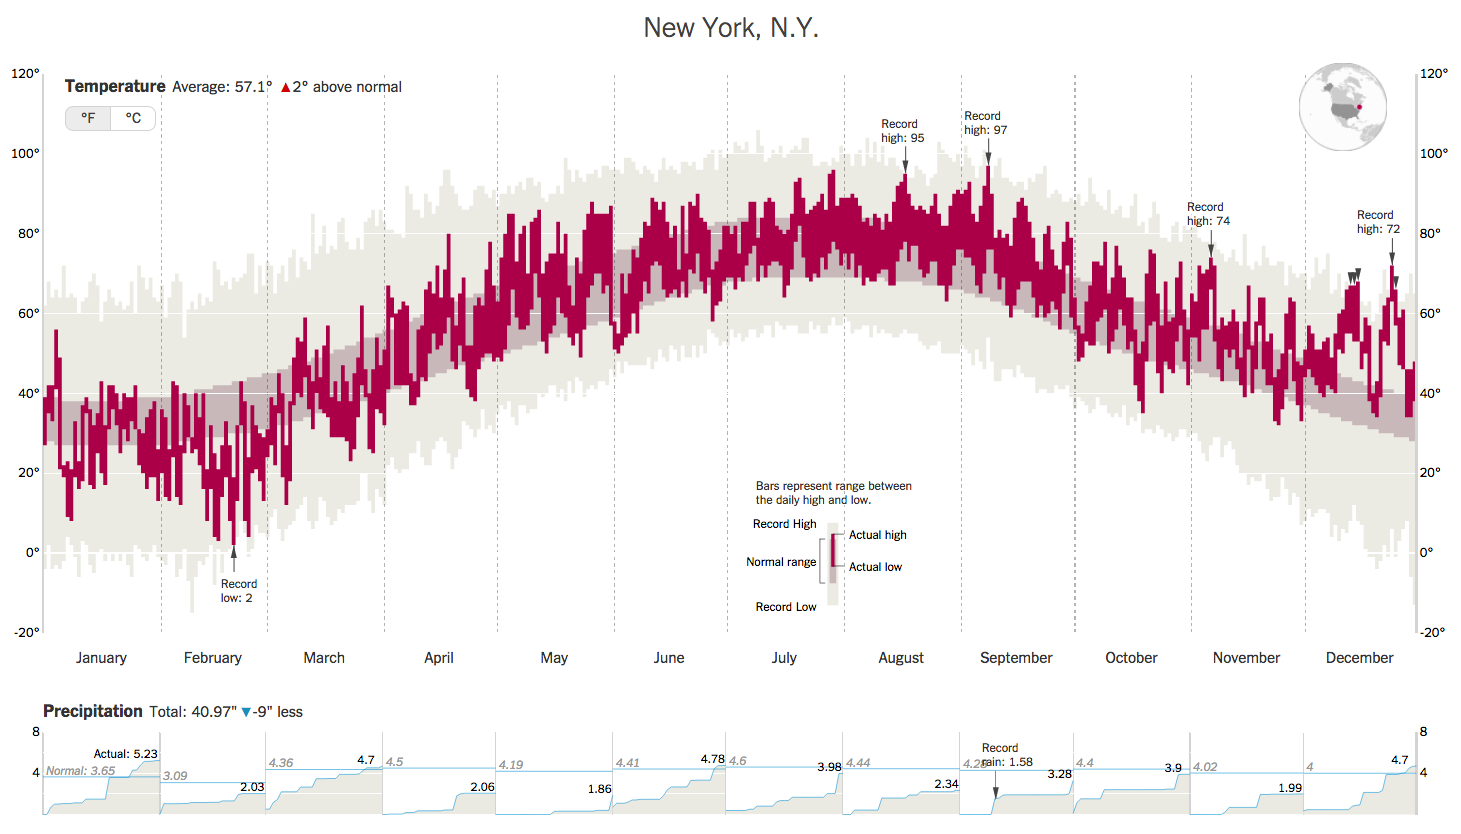
\includegraphics{images/clipboard-1399795317.png}

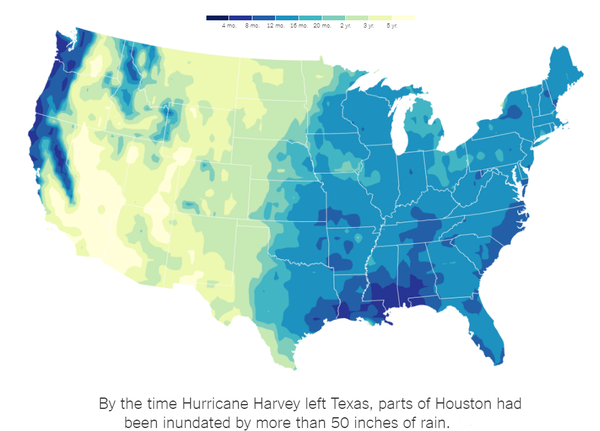
\includegraphics{images/clipboard-2893827168.png}

Enriquece tu gráfica con símbolos de color y texto para transmitir
información adicional.

\hypertarget{principio-3-aplica-los-principios-del-diseuxf1o-gruxe1fico}{%
\subsection{\texorpdfstring{\emph{Principio 3: Aplica los principios del
diseño
gráfico}}{Principio 3: Aplica los principios del diseño gráfico}}\label{principio-3-aplica-los-principios-del-diseuxf1o-gruxe1fico}}

\begin{enumerate}
\def\labelenumi{\arabic{enumi}.}
\tightlist
\item
  Es fácil identificar objetos por color.
\item
  Utiliza etiquetas directas en lugar de una leyenda.
\item
  Elementos como texto, líneas, y formas que tengan la misma naturaleza
  deben parecerse.
\item
  Equilibra gráficos y texto.
\item
  Ten cuidado con las opciones predeterminadas del software de
  visualización.
\item
  Usa un diseño de cuadrícula para organizar su visualización.
\end{enumerate}

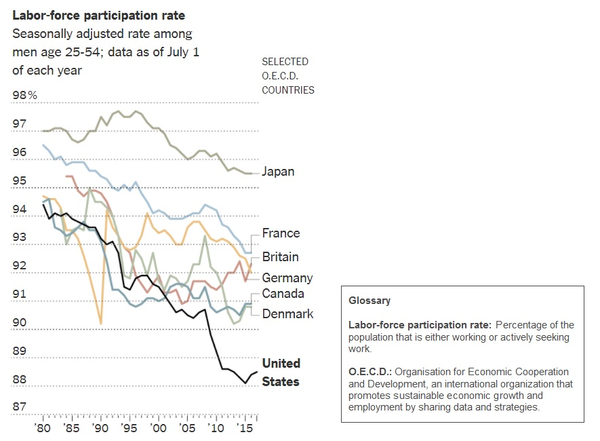
\includegraphics[width=5.04167in,height=3.53125in]{images/clipboard-2746624499.png}

No te limites a cosas simples. Enriquece tu gráfica con símbolos de
color para transmitir información adicional. Si es posible, agrega
contexto con marcadores y etiquetas de referencia.

También, agrega una leyenda a la grafica que describa las
características importantes y resuma sus conclusiones.

\hypertarget{section-2}{%
\subsection{}\label{section-2}}

\begin{quote}
``\emph{El mayor valor de una imagen es cuando nos obliga a notar lo que
nunca esperábamos ver.}'' John W. Tukey.
\end{quote}

\includegraphics{Introduccion_files/mediabag/John_Tukey.jpg}

Principios del diseño gráfico

\begin{enumerate}
\def\labelenumi{\arabic{enumi}.}
\item
  Es más fácil identificar objetos por color que por forma.
\item
  Cuando sea posible, utiliza etiquetas directas en lugar de una
  leyenda.
\item
  Elementos como texto, líneas, formas, etc., que tengan la misma
  naturaleza deben parecerse.
\item
  Haz un esfuerzo por lograr un equilibrio entre gráficos y texto.
\item
  Ten cuidado con las opciones predeterminadas del software de
  visualización.
\item
  Utiliza un diseño de cuadrícula para organizar su visualización.
\end{enumerate}

\hypertarget{actividad}{%
\section{Actividad}\label{actividad}}

\hypertarget{actividad-cooperative-mode}{%
\subsection{\texorpdfstring{Actividad (\emph{cooperative}
mode)}{Actividad (cooperative mode)}}\label{actividad-cooperative-mode}}

\begin{enumerate}
\def\labelenumi{\arabic{enumi}.}
\tightlist
\item
  Júntate con un compañero.
\item
  Encuentren un \textbf{buen} y un \textbf{mal} ejemplo de una
  visualización (gráficas) en linea.
\item
  Guarden las visualizaciones (por ejemplo, haciendo una captura de
  pantalla).
\item
  Escriban una crítica breve (3 a 4 enunciados) de cada visualización.
\item
  Suban un documento con sus criticas e imagenes en Canvas.
\end{enumerate}



\end{document}
